\documentclass[11pt]{article}

% AMS Packages
\usepackage{amsmath} 
\usepackage{amssymb} 
\usepackage{amsthm}
% Page dimensions
\usepackage[margin=1in]{geometry}
% Images
\usepackage[pdftex]{graphicx} 
% Enumerate package
\usepackage{enumitem} 
\usepackage{array} 
% Fancify pages
\usepackage{fancyhdr} 
% Convert captions on figures to bold font
\usepackage[labelfont=bf,textfont=md]{caption}
% Time New Roman font
\usepackage{times}

\usepackage{setspace} 
% SI Units in math type
\usepackage{siunitx}
\usepackage{textcomp} 
% Change sizes of sections
\usepackage{titlesec}
\titleformat{\section}{\normalfont\large\bfseries}{\thesection}{1em}{}
\titleformat{\subsection}{\normalfont\bfseries}{\thesubsection}{1em}{}
\titleformat{\subsubsection}{\normalfont\small\bfseries}{\thesubsubsection}{1em}{}
% Declare useful math operators
\DeclareMathOperator*{\argmin}{arg\,min}
\DeclareMathOperator*{\plim}{plim}
\DeclareMathOperator{\Tr}{Tr}

\usepackage{tikz}
\usetikzlibrary{shapes.geometric, arrows}

% title
\title{Synaptic weight diversity enhances encoding and decoding in the presence of common noise in a linear-nonlinear network}
\date{}
\begin{document}
	\maketitle
	
	\section{Introduction}
	\begin{figure}[ht]
	\centering
	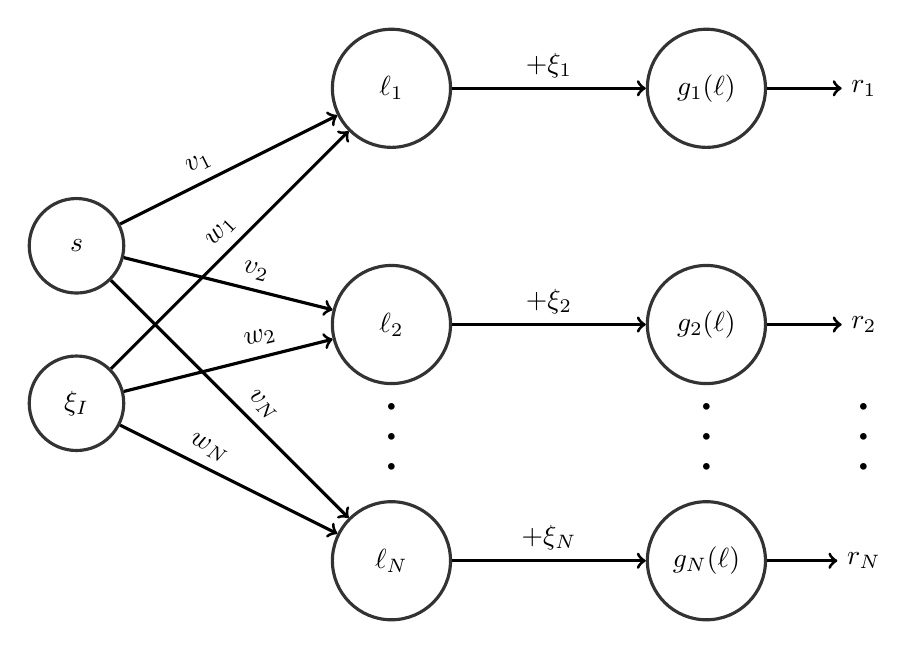
\begin{tikzpicture}
	\tikzstyle{main} = [circle, minimum size = 12mm, line width = 0.4mm, draw=black!80, node distance = 16mm]
	\tikzstyle{main2} = [circle, minimum size = 15mm, line width = 0.4mm, draw=black!80, node distance = 16mm]
	\node[main, fill = white!100] at (0, 1.) (s) {$s$};
	\node[main, fill = white!100] at (0, -1.) (inj) {$\xi_I$};
	\node[main2] at (4.,3.0)  (lin1) {$\ell_1$};
	\node[main2] at (4.,0.0)  (lin2) {$\ell_2$};
	\node[main2] at (4,-3.0) (linN) {$\ell_{N}$};
	
	\node[main2] at (8, 3.0) (nonlin1) {$g_1(\ell)$};
	\node[main2] at (8, 0.0) (nonlin2) {$g_2(\ell)$};
	\node[main2] at (8, -3.0) (nonlinN) {$g_N(\ell)$};
	
	\node at (10, 3.0) (r1) {$r_1$};
	\node at (10, 0.0) (r2) {$r_2$};
	\node at (10, -3.0) (rN) {$r_N$};
	
	\draw[->, line width = 0.4mm] (s) -- (lin1) node[midway, above left, sloped] {$v_1$};
	\draw[->, line width = 0.4mm] (s) -- (lin2) node[midway, above right, sloped] {$v_2$};
	\draw[->, line width = 0.4mm] (s) -- (linN) node[midway, above right, sloped] {$v_N$};
	
	\draw[->, line width = 0.4mm] (inj) -- (lin1) node[pos = 0.6, above left, sloped] {$w_1$};
	\draw[->, line width = 0.4mm] (inj) -- (lin2) node[pos = 0.8, above left, sloped] {$w_2$};
	\draw[->, line width = 0.4mm] (inj) -- (linN) node[midway, above left, sloped] {$w_N$};
	
	\draw[->, line width = 0.4mm] (lin1) -- (nonlin1) node[midway, above] {$+\xi_1$};
	\draw[->, line width = 0.4mm] (lin2) -- (nonlin2) node[midway, above] {$+\xi_2$};
	\draw[->, line width = 0.4mm] (linN) -- (nonlinN) node[midway, above] {$+\xi_N$};
	
	\draw[->, line width = 0.4mm] (nonlin1) -- (r1);
	\draw[->, line width = 0.4mm] (nonlin2) -- (r2);
	\draw[->, line width = 0.4mm] (nonlinN) -- (rN);
	
	\path (lin2) -- (linN) node [black, font=\Huge, midway, sloped] {$\dots$};
	\path (nonlin2) -- (nonlinN) node [black, font=\Huge, midway, sloped] {$\dots$};
	\path (r2) -- (rN) node [black, font=\Huge, midway, sloped] {$\dots$};	
	\end{tikzpicture}
	\caption{Linear-Nonlinear Network Architecture}
	\end{figure}
	\section{Fisher Information, Linear Stage}
	We can calculate the Fisher information after the first stage. 
	
	\section{Fisher Information, Quadratic Nonlinearity}
	\section{Mutual Information, Linear Stage}
	
	
	\appendix
	\newpage
	\section{Calculation of  Fisher Information, Linear Stage}
	All variability after the linear stage is Gaussian; thus, the Fisher information can be expressed in the form
	\begin{align}
		I_{F}(s) &= \mathbf{f}'(s)^T \boldsymbol{\Sigma}^{-1} (s) \mathbf{f}'(s) + \frac{1}{2}\Tr\left[\boldsymbol{\Sigma}'(s) \boldsymbol{\Sigma}^{-1}(s)\boldsymbol{\Sigma}'(s) \boldsymbol{\Sigma}^{-1}(s)\right]. \label{IF-gaussian}
	\end{align}
	Our immediate goal is to calculate $\mathbf{f}(s)$, the average response of the linear stage, and $\boldsymbol{\Sigma}$, the covariance between the responses. The output of the $i$th neuron after the linear stage is
	\begin{align}
		\ell_i &= v_i s + w_i \sigma_I \xi_I + \sigma_G\xi_i,
	\end{align}
	so that the average response as a function of $s$ is
	\begin{align}
		f_i(s) &= \langle \ell_i \rangle = v_i s.
	\end{align}
	Thus,
	\begin{align}
		\mathbf{f}(s) = \mathbf{v}s \Rightarrow \mathbf{f}'(s) = \mathbf{v}.
	\end{align}
	
	Meanwhile,
	\begin{align}
		\langle \ell_i \ell_j \rangle &= \langle (v_i s + w_i \sigma_I\xi_I + \sigma_G\xi_i) (v_j s + w_j \sigma_I\xi_I + \sigma_G\xi_j)\rangle \\
		&= v_i v_j s^2 + w_i w_j \sigma_I^2 + \sigma_G^2 \delta_{ij}
	\end{align}
	so that
	\begin{align}
		\Sigma_{ij} &= v_i v_j s^2 + w_i w_j \sigma_I^2 + \sigma_G^2 \delta_{ij} - v_i v_j s^2 \\
		&= \sigma_G^2 \delta_{ij} + w_i w_j \sigma_I^2 \\
		\Rightarrow \boldsymbol{\Sigma} &= \sigma_G^2 \mathbf{I} + \sigma_I^2\mathbf{ww}^T.
	\end{align}
	Notice that the covariance matrix does not depend on $s$, so the second term in equation \eqref{IF-gaussian} will vanish. We do, however, need the inverse covariance matrix for the first term:
	\begin{align}
		\boldsymbol{\Sigma}^{-1} &= \frac{1}{\sigma_G^2} \mathbf{I} - \frac{\sigma_I^2}{\sigma_G^4} \frac{\mathbf{ww}^T}{1+\frac{\sigma_I^2}{\sigma_G^2}||\mathbf{w}||^2}\\
		&= \frac{1}{\sigma_G^2}\left(\mathbf{I} - \frac{\sigma_I^2}{\sigma_G^2 + \sigma_I^2 |\mathbf{w}|^2}\mathbf{ww}^T\right).
	\end{align}
	
	Hence, the Fisher information is
	\begin{align}
		I_{F}(s) &= \frac{1}{\sigma_G^2}\mathbf{v}^T \left(\mathbf{I} - \frac{\sigma_I^2}{\sigma_G^2 + \sigma_I^2 |\mathbf{w}|^2}\mathbf{ww}^T\right) \mathbf{v} \\
		&= \frac{1}{\sigma_G^2} \left(|\mathbf{v}|^2 - \frac{\sigma_I^2 (\mathbf{v}\cdot\mathbf{w})^2}{\sigma_G^2 + \sigma_I^2 |\mathbf{w}|^2}\right) \\
		&= \frac{\sigma_G^2 |\mathbf{v}|^2 + \sigma_I^2 \left(|\mathbf{v}|^2|\mathbf{w}|^2 - (\mathbf{v}\cdot\mathbf{w})^2\right)}{\sigma_G^2 (\sigma_G^2 + \sigma_I^2 |\mathbf{w}|^2)}.
	\end{align}
	\newpage
	\section{Calculation of Fisher Information, Quadratic Nonlinearity}
	We repeat the calculation of the previous section, but after the nonlinear stage. In this case, we consider a quadratic nonlinearity. We calculate the linear Fisher information because it is simpler to do so analytically. 
	\begin{align}
	r_i &= (v_i s + w_i \sigma_I \xi_I + \sigma_G \xi_i)^2 \\
	&= v_i^2 s^2 + w_i^2 \sigma_I^2 \xi_I^2 +  \sigma_G^2 \xi_i^2 + 2s v_i w_i \sigma_I \xi_I + 2 v_i s \sigma_G \xi_i + w_i \sigma_I \sigma_G \xi_I \xi_i.
	\end{align}
	Thus, the average becomes 
	\begin{align}
	f_i(s) &= \langle r_i \rangle \\
	&= v_i^2 s^2 + w_i^2 \sigma_I^2 + \sigma_G^2,
	\end{align}
	which implies 
	\begin{align}
	\langle r_i \rangle  \langle r_j \rangle &= (v_i^2 s^2 + w_i^2 \sigma_I^2 + \sigma_G^2)(v_j^2 s^2 + w_j^2 \sigma_I^2 + \sigma_G^2)\\
	&= \sigma_G^4 + s^2 \sigma_G^2 (v_i^2 + v_j^2)  + \sigma_G^2 \sigma_I^2 (w_i^2 + w_j^2) + s^2 \sigma_I^2 (v_i^2 w_j^2 + v_j^2 w_i^2 ) + s^4 v_i^2 v_j^2+ \sigma_I^4 w_i^2 w_j^2
	\end{align}
	Next, the covariate becomes 
	\begin{align}
	\langle r_i r_j \rangle &= \left\langle \left(v_i^2 s^2 + w_i^2 \sigma_I^2 \xi_I^2 +  \sigma_G^2 \xi_i^2 + 2s v_i w_i \sigma_I \xi_I + 2 v_i s \sigma_G \xi_i + w_i \sigma_I \sigma_G \xi_I \xi_i\right) \right. \notag \\
	& \qquad \left. \left(v_j^2 s^2 + w_j^2 \sigma_I^2 \xi_I^2 +  \sigma_G^2 \xi_j^2 + 2s v_j w_j \sigma_I \xi_I + 2 v_j s \sigma_G \xi_j + w_i \sigma_I \sigma_G \xi_I \xi_i\right)\right\rangle \\
	&= \sigma_G^4 + s^2 \sigma_G^2 (v_i^2 + v_j^2) + \sigma_G^2 \sigma_I^2 (w_i^2 + w_j^2) + s^2 \sigma_I^2 (v_i^2 w_j^2 + v_j^2 w_i^2) + s^4 v_i^2 v_j^2 + 3\sigma_I^4 w_i^2 w_j^2 \notag \\
	& \qquad + 4s^2 \sigma_I^2 v_i v_j w_i w_j.
	\end{align}
	And so the off diagonal terms of the covariance matrix are 
	\begin{align}
	\langle r_i r_j \rangle - \langle r_i \rangle \langle r_j \rangle &= 2 \sigma_I^4 w_i^2 w_j^2 + 4s^2 \sigma_I^2 v_i v_j w_i w_j.
	\end{align}
	Lastly, the variance of $r_i$ (the on-diagonal terms in the covariance matrix) is given by 
	\begin{align}
	\text{Var}(r_i) &= \langle r_i^2 \rangle - \langle r_i\rangle^2 \\
	&= 3\sigma_G^4 + 6s^2\sigma_G^2  v_i^2  +6 \sigma_G^2 \sigma_I^2  w_i^2+  6s^2 \sigma_I^2 v_i^2 w_i^2+ s^4 v_i^4 + 3\sigma_I^4 w_i^4 \notag \\ 
	& \qquad -\left(v_i^2 s^2 + w_i^2 \sigma_I^2 + \sigma_G^2\right)^2 \\
	&= 2\sigma_I^4 w_i^4 + 4s^2 \sigma_I^2 v_i^2 w_i^2 + 2\sigma_G^2 + 4s^2 \sigma_G^2 v_i^2  + 4\sigma_G^2\sigma_I^2 w_i^2.
	\end{align}
	Thus, the total covariance, which takes the variance into consideration, is 
	\begin{align}
	\Sigma_{ij} &= 4 s^2 \sigma_I^2 v_i v_j w_i w_j + 2 \sigma_I^4 w_i^2 w_j^2 + \delta_{ij} \left(2 \sigma_G^4 + 4\sigma_G^2 (s^2 v_i^2 + \sigma_I^2 w_i^2)\right).
	\end{align}
	In vector notation, this is 
	\begin{align}
	\boldsymbol{\Sigma} &= 2\sigma_G^4 \mathbf{I} +4\sigma_G^2 s^2 \text{diag}(\mathbf{V}) + 4\sigma_G^2 \sigma_I^2 \text{diag}(\mathbf{W}) + 4s^2 \sigma_I^2 \mathbf{X}\mathbf{X}^T + 2 \sigma_I^4 \mathbf{W}\mathbf{W}^T.
	\end{align}
	We now proceed to the linear Fisher information:
	\begin{align}
	I_F(s) &= \mathbf{f}'(s)^T \boldsymbol{\Sigma}(s)^{-1} \mathbf{f}'(s)
	\end{align}
	for which we need the inverse of the covariance matrix. We will obtain this by repeated applications of the Sherman-Morrison formula. First, note that 
	\begin{align}
	\left(2\sigma_G^4 \mathbf{I} +4\sigma_G^2 s^2 \text{diag}(\mathbf{V}) + 4\sigma_G^2 \sigma_I^2 \text{diag}(\mathbf{W})\right)^{-1} &= \left(2\sigma_G^4 + 4\sigma_G^2 s^2 v_i^2 + 4\sigma_G^2 \sigma_I^2 w_i^2\right)^{-1}\delta_{ij}.
	\end{align}
	Thus,
	\begin{align}
	\mathbf{M}^{-1} &\equiv \left(2\sigma_G^4 \mathbf{I} +4\sigma_G^2 s^2 \text{diag}(\mathbf{V}) + 4\sigma_G^2 \sigma_I^2 \text{diag}(\mathbf{W}) + 4s^2 \sigma_I^2 \mathbf{X}\mathbf{X}^T\right)^{-1} \\
	&= \left(2\sigma_G^4 + 4\sigma_G^2 s^2 v_i^2 + 4\sigma_G^2 \sigma_I^2 w_i^2\right)^{-1}\delta_{ij} \notag \\
	& - \frac{1}{1 + \sum_i\frac{4s^2\sigma_I^2 v_i^2 w_i^2}{2\sigma_G^4 + 4\sigma_G^2 s^2 v_i^2 + 4\sigma_G^2 \sigma_I^2 w_i^2}}\frac{(4s^2 \sigma_I^2 v_i v_j w_i w_j)}{\left(2\sigma_G^4 + 4\sigma_G^2 s^2 v_i^2 + 4\sigma_G^2 \sigma_I^2 w_i^2\right)\left(2\sigma_G^4 + 4\sigma_G^2 s^2 v_j^2 + 4\sigma_G^2 \sigma_I^2 w_j^2\right)} \\
	&= \left(2\sigma_G^4 + 4\sigma_G^2 s^2 v_i^2 + 4\sigma_G^2 \sigma_I^2 w_i^2\right)^{-1}\delta_{ij} \notag \\
	& - \frac{2s^2\sigma_I^2}{\sigma_G^4 +2s^2\sigma_I^2 \sigma_G^2\displaystyle\sum_i\frac{v_i^2 w_i^2}{\sigma_G^2+ 2s^2 v_i^2 + 2 \sigma_I^2 w_i^2}} \frac{ v_i v_j w_i w_j}{\left(\sigma_G^2 + 2s^2 v_i^2 + 2 \sigma_I^2 w_i^2\right)\left(\sigma_G^2 + 2 s^2 v_j^2 + 2\sigma_I^2 w_j^2\right)}.
	\end{align}
	Lastly, we have 
	\begin{align}
	\boldsymbol{\Sigma}^{-1} &= (\mathbf{M} + 2\sigma_I^4 \mathbf{W}\mathbf{W}^T)^{-1} \\
	&= \mathbf{M}^{-1} - \frac{\mathbf{M}^{-1} (2\sigma_I^4 \mathbf{W}\mathbf{W}^T) \mathbf{M}^{-1}}{1 + 2\sigma_I^4 \mathbf{W}^T\mathbf{M}^{-1}\mathbf{W}} \\
	&= \mathbf{M}^{-1} - \frac{2\sigma_I^4}{1 + 2\sigma_I^4 \mathbf{W}^T\mathbf{M}^{-1} \mathbf{W}} \mathbf{M}^{-1}\mathbf{W}\mathbf{W}^T\mathbf{M}^{-1}.
	\end{align}
	Note that
	\begin{align}
	\mathbf{f}'(s) &= 2 s \mathbf{V},
	\end{align}
	so the Fisher information is
	\begin{align}
	I_F(s) &= 4s^2 \left(\mathbf{V}^T \mathbf{M}^{-1} \mathbf{V} - \frac{2\sigma_I^4}{1 + 2\sigma_I^4 \mathbf{W}^T\mathbf{M}^{-1} \mathbf{W}} \mathbf{V}^T \mathbf{M}^{-1} \mathbf{W} \mathbf{W}^T \mathbf{M}^{-1}\mathbf{V}\right) \\
	&= 4s^2 \left(\mathbf{V}^T \mathbf{M}^{-1} \mathbf{V}-  \frac{2\sigma_I^4}{1 + 2\sigma_I^4 \mathbf{W}^T\mathbf{M}^{-1} \mathbf{W}} \left(\mathbf{V}^T\mathbf{M}^{-1} \mathbf{W}\right)^{2}\right).
	\end{align}
	Before we proceed, we'll define the notation 
	\begin{align}
	\left\{v, w\right\}_{m,n} &= \sum_i \frac{v_i^m w_i^n}{\sigma_G^2 + 2s^2 v_i^2 + 2\sigma_I^2 w_i^2}.
	\end{align}
	Thus,
	\begin{align}
	\mathbf{V}^T \mathbf{M}^{-1}\mathbf{V} &= \frac{1}{2\sigma_G^2}\sum_i \frac{v_i^4}{\sigma_G^2 + 2s^2 v_i^2  +2\sigma_I^2 w_i^2} \notag \\
	&- \frac{2s^2\sigma_I^2}{\sigma_G^4 + 2s^2 \sigma_I^2 \sigma_G^2 \left\{v,w\right\}_{2,2}} \left(\sum_i\frac{v_i^3 w_i}{\sigma_G^2 + 2s^2 v_i^2 + 2 \sigma_I^2 w_i^2}\right)^2 \\
	&= \frac{1}{\sigma_G^2}\left\{v,w\right\}_{4,0} - \frac{2s^2 \sigma_I^2}{\sigma_G^4 + 2s^2 \sigma_I^2 \sigma_G^2 \left\{v,w\right\}_{2,2}} \left\{v,w\right\}_{3,1}^2.
	\end{align}
	Furthermore,
	\begin{align}
	\mathbf{W}^T \mathbf{M}^{-1}\mathbf{W}  &= \frac{1}{2\sigma_G^2}\left\{v,w\right\}_{0,4} - \frac{2s^2\sigma_I^2}{\sigma_G^4 + 2s^2 \sigma_I^2 \sigma_G^2 \left\{v,w\right\}_{2,2}} \left\{v,w\right\}_{1,3}^2
	\end{align}
	and lastly
	\begin{align}
	\mathbf{V}^T \mathbf{M}^{-1} \mathbf{W} &= \frac{1}{2\sigma_G^2}\left\{v,w\right\}_{2,2} - \frac{2s^2\sigma_I^2}{\sigma_G^4 + 2s^2\sigma_I^2 \sigma_G^2\left\{v,w\right\}_{2,2}} \left\{v,w\right\}_{1,3}\left\{v,w\right\}_{3,1}.
	\end{align}
	Thus, the Fisher information is 
	\begin{align}
	I_F(s) &= 4s^2 \left(\frac{1}{\sigma_G^2}\left\{v, w\right\}_{4,0} - \frac{2s^2 \sigma_I^2}{\sigma_G^2 + 2s^2 \sigma_G^2 \sigma_I^2 \left\{v,w\right\}_{2,2}} \left\{v,w\right\}_{3,1}^2  \right. \notag \\
	&\left. + \frac{\sigma_G^2 \sigma_I^4 \left\{v,w\right\}_{2,2} + 2s^2 \sigma_I^6 (\left\{v,w\right\}_{2,2} - 2 \left\{v,w\right\}_{1,3} \left\{v,w\right\}_{3,1})}{\sigma_G^4  + \sigma_G^2 (\sigma_I^4 \left\{v,w\right\}_{0,4} + 2s^2 \sigma_I^2 \left\{v,w\right\}_{2,2}) + 2s^2 \sigma_I^6 (\left\{v,w\right\}_{0,4} \left\{v,w\right\}_{2,2} - 2 \left\{v,w\right\}_{1,3}^2)}\right)
	\end{align}
	\newpage
	\section{Calculation of Conditional and Marginal Probability Distributions}
	We present the calculation of the conditional and marginal probability distributions after the linear stage of computation. Recall that the output of the $i$th neuron in the linear stage can be written as
	\begin{align}
		\ell_i &= v_i s + w_i \sigma_I \xi_I + \sigma_G\xi_i
	\end{align}
	and thus the overall population can be written as 
	\begin{align}
		\boldsymbol{\ell} &= \mathbf{v} s + \mathbf{w} \sigma_I \xi_I + \sigma_G \boldsymbol{\xi}.
	\end{align}
	
	\subsection{Conditional Distribution $P[\boldsymbol{\ell}|s]$}
	Conditioning on the stimulus and injected noise value establishes independence between the neural activity $\ell_i$. Thus, we obtain $P[\boldsymbol{\ell}|s]$ by marginalizing the distribution $P[\boldsymbol{\ell}|s,\xi_I]$ over the injected noise $\xi_I$:
	\begin{align}
	P[\boldsymbol{\ell}|s] &= \int P[\boldsymbol{\ell}|s, \xi_I] P[\xi_I]d\xi_I \\
	&= \int d\xi_I  \frac{1}{\sqrt{2\pi}} \exp(-\xi_I^2/2) \prod_{i=1}^N P[\ell_i|s,\xi_I] \\
	&=  \frac{1}{\sqrt{2\pi}} \int d\xi_I   \exp(-\xi_I^2/2) \prod_{i=1}^N \frac{1}{\sqrt{2\pi \sigma_G^2}} \exp\left(-\frac{\left(\ell_i - (v_i s + \sigma_I w_i \xi_I)\right)^2}{2\sigma_G^2}\right) \\
	&= \frac{1}{(2\pi)^{(N+1)/2}\sigma_G^N} \int d\xi_I \exp(-\xi_I^2/2) \exp\left(-\frac{1}{2\sigma_G^2}\sum_{i=1}^N \left(\ell_i - (v_i s + \sigma_I w_i \xi_I)\right)^2\right) \\
	&= \frac{1}{(2\pi)^{(N+1)/2}\sigma_G^N} \int d\xi_I \exp(-\xi_I^2/2) \notag \\
	& \qquad \times \exp\left(-\frac{1}{2\sigma_G^2}\sum_{i=1}^N \ell_i^2 -2\ell_i (v_i s + \sigma_I w_i \xi_I) + (v_i s + \sigma_I w_i \xi_I)^2\right) \\
	&= \frac{1}{(2\pi)^{(N+1)/2}\sigma_G^N} \exp\left(-\frac{1}{2\sigma_G^2}\sum_{i=1}^N \ell_i^2\right)\exp\left(\frac{s}{\sigma_G^2}\sum_{i=1}^N \ell_i v_i \right)\exp\left(-\frac{1}{2\sigma_G^2}s^2 |\mathbf{v}|^2\right) \notag \\
	&\times \int d\xi_I\exp\left[-\frac{1}{2}\left(1+\frac{\sigma_I^2}{\sigma_G^2} |\mathbf{w}|^2\right)\xi_I^2 +\frac{\sigma_I}{\sigma_G^2}\left( \sum_{i=1}^N \ell_i w_i - s v_i w_i\right)\xi_I \right] \\
	&=  \frac{1}{(2\pi)^{(N+1)/2}\sigma_G^N}\exp\left(-\frac{1}{2\sigma_G^2}\sum_{i=1}^N \ell_i^2\right)\exp\left(\frac{s}{\sigma_G^2}\sum_{i=1}^N \ell_i v_i \right)\exp\left(-\frac{1}{2\sigma_G^2}s^2 |\mathbf{v}|^2\right) \notag \\
	&\qquad \times \frac{\sqrt{2\pi \sigma_G^2}}{\sqrt{\sigma_G^2 + \sigma_I^2 \left\{w\right\}_2}}\exp\left[\frac{\sigma_I^2\left(\displaystyle\sum_{i=1}^N \ell_i w_i - s  v_i w_i \right)^2}{2 \sigma_G^2 (\sigma_G^2 + \sigma_I^2 \left\{w\right\}_2)}\right],
	\end{align}
	which we can write concisely as
	\begin{align}
		P[\boldsymbol{\ell}|s] &= \frac{1}{\sigma_G^{N-1} \sqrt{(2\pi)^N(\sigma_G^2 + \sigma_I^2 ||\mathbf{w}||^2)}} \exp\left[-\frac{1}{2\sigma_G^2} (\boldsymbol{\ell} - \mathbf{v}s)^T\left(\mathbf{I} - \frac{\sigma_I^2 \mathbf{ww}^T}{\sigma_G^2 + \sigma_I^2 ||\mathbf{w}||^2}\right) (\boldsymbol{\ell} - \mathbf{v}s) \right].
	\end{align}
	\subsection{Marginal Distribution $P[\boldsymbol{\ell}]$}
	We can calculate the marginal distribution either by summing the three Gaussians $\mathbf{v}s$, $\mathbf{w} \sigma_I \xi_I$, and $\sigma_G\boldsymbol{\xi}$, or by marginalizing the conditional probability distribution. 
	
	The marginal distribution is 
	\begin{align}
		 P[\boldsymbol{\ell}] = \frac{1}{\sigma_G^{N-2} \sqrt{(2\pi)^N \kappa}} &\exp\left[-\frac{1}{2\sigma_G^2} \boldsymbol{\ell}^T  \left(\mathbf{I} -\frac{\sigma_I^2 (\sigma_G^2 + \sigma_S^2 |\mathbf{v}|^2)}{\kappa} \mathbf{ww}^T + \frac{\sigma_I^2 \sigma_S^2 (\mathbf{v}\cdot\mathbf{w})}{\kappa}\mathbf{wv}^T \right. \right. \notag \\
		&\left. \left. \qquad \qquad \qquad \qquad  + \frac{\sigma_I^2 \sigma_S^2 (\mathbf{v}\cdot\mathbf{w})}{\kappa}\mathbf{wv}^T- \frac{\sigma_S^2 (\sigma_G^2 +\sigma_I^2 |\mathbf{w}|^2)}{\kappa} \mathbf{vv}^T\right) \boldsymbol{\ell}\right], \label{marginal-1}
	\end{align}
	where we note that 
	\begin{align}
		\kappa &= (\sigma_G^2 + \sigma_I^2 |\mathbf{w}|^2)(\sigma_G^2 + \sigma_S^2 |\mathbf{v}|^2) - \sigma_I^2 \sigma_S^2 (\mathbf{v}\cdot\mathbf{w})^2.
	\end{align}
	We can write the marginal compactly as 
	\begin{align}
		P[\boldsymbol{\ell}] &= \frac{1}{\sigma_G^{N-2} \sqrt{(2\pi)^N \kappa}} \exp\left[-\frac{1}{2\sigma_G^2} \boldsymbol{\ell}^T \left(\mathbf{I} + A_1 \mathbf{ww}^T + A_2 (\mathbf{wv}^T +\mathbf{vw}^T) + A_3 \mathbf{vv}^T\right) \boldsymbol{\ell}\right], \label{marginal-2}\\
		&= \frac{1}{\sigma_G^{N-2} \sqrt{(2\pi)^N \kappa}} \exp\left[-\boldsymbol{\ell}^T \mathbf{A} \boldsymbol{\ell}\right]
	\end{align}
	where
	\begin{align}
		A_1 &= -\frac{\sigma_I^2 (\sigma_G^2 + \sigma_S^2 |\mathbf{v}|^2)}{\kappa} \\
		A_2 &= \frac{2 \sigma_I^2 \sigma_S^2 (\mathbf{v}\cdot\mathbf{w})}{\kappa} \\
		A_3 &= -\frac{\sigma_S^2 (\sigma_G^2 + \sigma_I^2 |\mathbf{w}|^2)}{\kappa}.
	\end{align}
	Noting, however, that the marginal is effectively a multivariate Gaussian, we know that
	\begin{align}
		P[\boldsymbol{\ell}] &= \frac{1}{\sqrt{(2\pi)^N \det\boldsymbol{\Sigma}}} \exp\left[-\frac{1}{2} \boldsymbol{\ell}^T \boldsymbol{\Sigma}^{-1} \boldsymbol{\ell}\right]
	\end{align}
	where 
	\begin{align}
		\boldsymbol{\Sigma}&= \sigma_G^2 \mathbf{I} + \sigma_S^2 \mathbf{vv}^T + \sigma_I^2 \mathbf{ww}^T,
	\end{align}
	or the covariance matrix comprised from summing the random variables $\mathbf{v}s+\mathbf{w}\sigma_I\xi_I + \sigma_G\boldsymbol{\xi}$. This implies that 
	\begin{align}
		\mathbf{A} &= \frac{1}{2} \boldsymbol{\Sigma}^{-1} \\
		\Rightarrow \mathbf{A}^{-1} &= 2 \boldsymbol{\Sigma} = 2\left(\sigma_G^2 \mathbf{I} + \sigma_S^2 \mathbf{vv}^T + \sigma_I^2 \mathbf{ww}^T\right).
	\end{align}
	Furthermore, 
	\begin{align}
		\det \mathbf{\mathbf{A}} &= \frac{1}{2^N} \det \boldsymbol{\Sigma}^{-1} = \frac{1}{2^N \sigma_G^{2N-4} \kappa}.
	\end{align}
	\newpage
	
	\section{Calculation of Mutual Information, Linear Stage}
	Here we present the calculation of mutual information $I[s, \boldsymbol{\ell}]$ between the stimulus $s$ and the output of the linear stage $\boldsymbol{\ell}$.
	
	\subsection{Setting up the Mutual Information Integral}
	The mutual information is given by 
	\begin{align}
		I[s,\boldsymbol{\ell}] &= \int d\boldsymbol{\ell} ds P[s] P[\boldsymbol{\ell}|s] \log \frac{P[\boldsymbol{\ell}|s]}{P[\boldsymbol{\ell}]}.
	\end{align}
	The ratio between the conditional and marginal distribution is given by 
	\begin{align}
		\frac{P[\boldsymbol{\ell}|s]}{P[\boldsymbol{\ell}]} &= \frac{1}{\sigma_G}\sqrt{\frac{\kappa}{\sigma_G^2 + \sigma_I^2 |\mathbf{w}|^2}} \exp\left[\frac{1}{2\sigma_G^2} \boldsymbol{\ell}^T \left(A_1 \mathbf{ww}^T + A_2 \mathbf{wv}^T + A_2 \mathbf{vw}^T+ A_3 \mathbf{vv}^T\right)\boldsymbol{\ell}\right] \notag \\
		&\times \exp\left[\frac{1}{2\sigma_G^2} \boldsymbol{\ell}^T \left(\frac{\sigma_I^2 \mathbf{ww}^T}{\sigma_G^2 + \sigma_I^2 |\mathbf{w}|^2}\right)\boldsymbol{\ell}\right]\exp\left[\frac{1}{2\sigma_G^2} \boldsymbol{\ell}^T\left(\mathbf{I} - \frac{\sigma_I^2 \mathbf{ww}^T}{\sigma_G^2 + \sigma_I^2 |\mathbf{w}|^2}\right)\mathbf{v}s\right] \notag \\
		&\times \exp\left[\frac{1}{2\sigma_G^2} s\mathbf{v}^T\left(\mathbf{I} - \frac{\sigma_I^2 \mathbf{ww}^T}{\sigma_G^2 + \sigma_I^2 |\mathbf{w}|^2}\right) \boldsymbol{\ell}\right]\exp\left[-\frac{1}{2\sigma_G^2} s^2 \mathbf{v}^T \left(\mathbf{I} - \frac{\sigma_I^2 \mathbf{ww}^T}{\sigma_G^2 + \sigma_I^2 |\mathbf{w}|^2}\right) \mathbf{v}\right] \\
		&=  \frac{1}{\sigma_G}\sqrt{\frac{\kappa}{\sigma_G^2 + \sigma_I^2 |\mathbf{w}|^2}} \exp\left[\frac{1}{2\sigma_G^2}\boldsymbol{\ell}^T\left(-\frac{\sigma_I^4 \sigma_S^2(\mathbf{v}\cdot\mathbf{w})^2}{\kappa(\sigma_G^2 + \sigma_I^2 |\mathbf{w}|^2)}\mathbf{ww}^T + A_2 \mathbf{wv}^T + A_3 \mathbf{vv}^T\right)\boldsymbol{\ell}\right] \notag \\
		&\times \exp\left[\frac{s (\boldsymbol{\ell} \cdot \mathbf{v})}{\sigma_G^2}\right]\exp\left[-\frac{s\sigma_I^2 (\boldsymbol{\ell}\cdot \mathbf{w})(\mathbf{v}\cdot\mathbf{w})}{\sigma_G^2 (\sigma_G^2 + \sigma_I^2 |\mathbf{w}|^2)}\right]\exp\left[-\frac{s^2}{2\sigma_G^2} \left(|\mathbf{v}|^2 -\frac{\sigma_I^2 (\mathbf{v}\cdot\mathbf{w})^2}{\sigma_G^2 + \sigma_I^2 |\mathbf{w}|^2}\right)\right].
	\end{align}
	Taking the logarithm of this gives us
	\begin{align}
		\log \frac{P[\boldsymbol{\ell}|s]}{P[\boldsymbol{\ell}]} &= \log \left(\frac{1}{\sigma_G}\sqrt{\frac{\kappa}{\sigma_G^2 + \sigma_I^2 |\mathbf{w}|^2}}\right) \notag \\
		&+ \frac{1}{2\sigma_G^2}\boldsymbol{\ell}^T\left(-\frac{\sigma_I^4 \sigma_S^2(\mathbf{v}\cdot\mathbf{w})^2}{\kappa(\sigma_G^2 + \sigma_I^2 |\mathbf{w}|^2)}\mathbf{ww}^T + A_2 \mathbf{wv}^T + A_2 \mathbf{vw}^T+ A_3 \mathbf{vv}^T\right)\boldsymbol{\ell} \notag \\
		&+ \frac{1}{2\sigma_G^2} \left[-s^2 \left(|\mathbf{v}|^2 -\frac{\sigma_I^2 (\mathbf{v}\cdot\mathbf{w})^2}{\sigma_G^2 + \sigma_I^2 |\mathbf{w}|^2}\right) + 2s \left((\boldsymbol{\ell} \cdot\mathbf{v}) - \frac{\sigma_I^2 (\boldsymbol{\ell}\cdot \mathbf{w})(\mathbf{v}\cdot\mathbf{w})}{\sigma_G^2 (\sigma_G^2 + \sigma_I^2 |\mathbf{w}|^2)}\right)\right].
	\end{align}
	The log-ratio consists of three terms: a constant, a term that depends strictly on $\boldsymbol{\ell}$, and a term that depends on both $\boldsymbol{\ell}$ and $s$. 
	Thus, we split up the mutual information as follows:
	\begin{gather}
		 I = I_1 + I_2 + I_3 \\
		 =\int d\boldsymbol{\ell} ds P[s] P[\boldsymbol{\ell}|s] \log \left(\frac{1}{\sigma_G}\sqrt{\frac{\kappa}{\sigma_G^2 + \sigma_I^2 |\mathbf{w}|^2}}\right) \notag \\
		+ \int d\boldsymbol{\ell} ds P[s]P[\boldsymbol{\ell}|s] \left[\frac{1}{2\sigma_G^2}\boldsymbol{\ell}^T\left(-\frac{\sigma_I^4 \sigma_S^2(\mathbf{v}\cdot\mathbf{w})^2}{\kappa(\sigma_G^2 + \sigma_I^2 |\mathbf{w}|^2)}\mathbf{ww}^T + A_2 \mathbf{wv}^T + A_2 \mathbf{vw}^T + A_3 \mathbf{vv}^T\right)\boldsymbol{\ell}\right] \notag \\
		+ \int d\boldsymbol{\ell}ds P[s] P[\boldsymbol{\ell}|s] \times  \frac{1}{2\sigma_G^2} \left[-s^2 \left(|\mathbf{v}|^2 -\frac{\sigma_I^2 (\mathbf{v}\cdot\mathbf{w})^2}{\sigma_G^2 + \sigma_I^2 |\mathbf{w}|^2}\right) + 2s \left((\boldsymbol{\ell} \cdot\mathbf{v}) - \frac{\sigma_I^2 (\boldsymbol{\ell}\cdot \mathbf{w})(\mathbf{v}\cdot\mathbf{w})}{\sigma_G^2 (\sigma_G^2 + \sigma_I^2 |\mathbf{w}|^2)}\right)\right].
	\end{gather}
	The first term, call it $I_1$, is easy: the integral will marginalize out both probability distributions, and we are left with
	\begin{align}
		I_1 &= \log \left(\frac{1}{\sigma_G}\sqrt{\frac{\kappa}{\sigma_G^2 + \sigma_I^2 |\mathbf{w}|^2}}\right).
	\end{align}
	In the second term, $I_2$, we can evaluate the $s$ integral for free because the attached term only depends on $\boldsymbol{\ell}$. So,
	\begin{align}
		I_2 &= \int d\boldsymbol{\ell}\left[\frac{1}{2\sigma_G^2}\boldsymbol{\ell}^T\left(-\frac{\sigma_I^4 \sigma_S^2(\mathbf{v}\cdot\mathbf{w})^2}{\kappa(\sigma_G^2 + \sigma_I^2 |\mathbf{w}|^2)}\mathbf{ww}^T + A_2 \mathbf{wv}^T + A_2 \mathbf{vw}^T+ A_3 \mathbf{vv}^T\right)\boldsymbol{\ell}\right]  P[\boldsymbol{\ell}] \\
		&= \frac{1}{2\sigma_G^N\sqrt{(2\pi)^N \kappa}} \int d\boldsymbol{\ell} \ \boldsymbol{\ell}^T\left(B_1 \mathbf{ww}^T + A_2\mathbf{wv}^T+ A_2\mathbf{vw}^T+ A_3\mathbf{vv}^T\right)\boldsymbol{\ell} \exp\left[-\boldsymbol{\ell}^T \mathbf{A} \boldsymbol{\ell}\right] \\
		&= \frac{1}{2\sigma_G^N \sqrt{(2\pi)^N \kappa}} \int d\boldsymbol{\ell} \left[\boldsymbol{\ell}^T \mathbf{B} \boldsymbol{\ell}\right]  \exp\left[-\boldsymbol{\ell}^T \mathbf{A} \boldsymbol{\ell}\right]
	\end{align}
	where 
	\begin{align}
		\mathbf{B} &= B_1 \mathbf{ww}^T + A_2\mathbf{wv}^T + A_2\mathbf{vw}^T+ A_3\mathbf{vv}^T.
	\end{align}
	This integral can be evaluated with the identity
	\begin{align}
		\int d\boldsymbol{\ell}  \left[\boldsymbol{\ell}^T \mathbf{C}_1 \boldsymbol{\ell} \right] \exp\left[-\boldsymbol{\ell}^T \mathbf{C}_2 \boldsymbol{\ell}\right] &= \sqrt{\frac{\pi^N}{\det \mathbf{C}_2}}\Tr(\mathbf{C}_1 \mathbf{C}_2^{-1}).
	\end{align}
	Thus, 
	\begin{align}
		I_2 &= \frac{1}{2\sigma_G^N \sqrt{(2\pi)^N \kappa}}\sqrt{\frac{\pi^N}{\det \mathbf{A}}}\Tr(\mathbf{B} \mathbf{A}^{-1}) \\
		&= \frac{1}{2\sigma_G^N} \sqrt{\frac{2^N \sigma_G^{2N-4} \kappa}{2^N \kappa}} \Tr (\mathbf{B}\mathbf{A}^{-1}) \\
		&= \frac{1}{2\sigma_G^2} \Tr(\mathbf{B}\mathbf{A}^{-1}).
	\end{align}
	
	As for the last term, we have
	\begin{align}
		I_3 &= \frac{1}{2\sigma_G^2}\int d\boldsymbol{\ell} ds P[s] P[\boldsymbol{\ell}|s] \left[-s^2 \left(|\mathbf{v}|^2 -\frac{\sigma_I^2 (\mathbf{v}\cdot\mathbf{w})^2}{\sigma_G^2 + \sigma_I^2 |\mathbf{w}|^2}\right) + 2s \left((\boldsymbol{\ell} \cdot\mathbf{v}) - \frac{\sigma_I^2 (\boldsymbol{\ell}\cdot \mathbf{w})(\mathbf{v}\cdot\mathbf{w})}{\sigma_G^2 (\sigma_G^2 + \sigma_I^2 |\mathbf{w}|^2)}\right)\right] \\
		&= \frac{1}{2\sigma_G^2} \frac{1}{\sqrt{2\pi \sigma_S^2}} \frac{1}{\sigma_G^{N-1} \sqrt{(2\pi)^N(\sigma_G^2 + \sigma_I^2 ||\mathbf{w}||^2)}} \int d\boldsymbol{\ell} \exp\left[-\frac{1}{2\sigma_G^2} \boldsymbol{\ell}^T \left(\mathbf{I} - \frac{\sigma_I^2 \mathbf{ww}^T}{\sigma_G^2 + \sigma_I^2 |\mathbf{w}|^2}\right)\boldsymbol{\ell}\right] \notag \\
		&\times \int ds \exp\left[\frac{s (\boldsymbol{\ell} \cdot \mathbf{v})}{\sigma_G^2}\right]\exp\left[-\frac{s\sigma_I^2 (\boldsymbol{\ell}\cdot \mathbf{w})(\mathbf{v}\cdot\mathbf{w})}{\sigma_G^2 (\sigma_G^2 + \sigma_I^2 |\mathbf{w}|^2)}\right]\exp\left[-\frac{s^2}{2\sigma_G^2} \left(|\mathbf{v}|^2 -\frac{\sigma_I^2 (\mathbf{v}\cdot\mathbf{w})^2}{\sigma_G^2 + \sigma_I^2 |\mathbf{w}|^2}\right)\right] \exp\left[-\frac{s^2}{2\sigma_S^2}\right]\notag \\
		&\times \left[-s^2 \left(|\mathbf{v}|^2 -\frac{\sigma_I^2 (\mathbf{v}\cdot\mathbf{w})^2}{\sigma_G^2 + \sigma_I^2 |\mathbf{w}|^2}\right) + 2s \left((\boldsymbol{\ell} \cdot\mathbf{v}) - \frac{\sigma_I^2 (\boldsymbol{\ell}\cdot \mathbf{w})(\mathbf{v}\cdot\mathbf{w})}{\sigma_G^2 + \sigma_I^2 |\mathbf{w}|^2}\right)\right] \\
		&= -\frac{\sigma_S^2}{2(2\pi)^{N/2} \sigma_G^N \kappa^{5/2} (\sigma_G^2 + \sigma_I^2 ||\mathbf{w}||^2)}\int d\boldsymbol{\ell}(C + \boldsymbol{\ell}^T \mathbf{D} \boldsymbol{\ell})\exp(-\boldsymbol{\ell}^T \mathbf{A} \boldsymbol{\ell})
	\end{align}
	where
	\begin{align}
	\mathbf{D} &= \gamma \left(-\sigma_I^4 (\mathbf{v}\cdot\mathbf{w})^2\mathbf{ww}^T+ \sigma_I^2 (\sigma_G^2 + \sigma_I^2 ||\mathbf{w}||^2)(\mathbf{v} \cdot \mathbf{w})\left(\mathbf{wv}^T + \mathbf{vw}^T\right) -(\sigma_G^2 + \sigma_I^2 ||\mathbf{w}||^2)^2 \mathbf{vv}^T\right)\\
	\gamma &= (2\sigma_G^2 + \sigma_S^2 ||\mathbf{v}||^2)(\sigma_G^2 + \sigma_I^2 ||\mathbf{w}||^2) - \sigma_I^2 \sigma_S^2 (\mathbf{v}\cdot \mathbf{w})^2.
	\end{align}
	and 
	\begin{align}
	C &= \kappa \sigma_G^2 (\sigma_G^2 + \sigma_I^2 ||\mathbf{w}||^2)(\sigma_G^2 ||\mathbf{v}||^2 + \sigma_I^2(||\mathbf{v}||^2 ||\mathbf{w}||^2 - (\mathbf{v}\cdot \mathbf{w})^2)).
	\end{align}
	Evaluating the integral with the above identity gives us
	\begin{align}
		I_3 &= -\frac{\sigma_S^2}{2(2\pi)^{N/2} \sigma_G^N \kappa^{5/2} (\sigma_G^2 + \sigma_I^2 ||\mathbf{w}||^2)}\sqrt{\frac{\pi^N}{\det \mathbf{A}}}\left[C + \Tr (\mathbf{D}\mathbf{A}^{-1})\right] \\
		&= -\frac{\sigma_S^2}{2\sigma_G^2 \kappa^2 (\sigma_G^2 + \sigma_I^2 ||\mathbf{w}||^2)}\left[C + \Tr (\mathbf{D}\mathbf{A}^{-1})\right] \\
		&= -\frac{\sigma_S^2}{2\kappa}(\sigma_G^2 ||\mathbf{v}||^2 + \sigma_I^2(||\mathbf{v}||^2 ||\mathbf{w}||^2 - (\mathbf{v}\cdot \mathbf{w})^2)) \notag \\
		&\qquad -\frac{\sigma_S^2}{2\sigma_G^2 \kappa^2 (\sigma_G^2 + \sigma_I^2 ||\mathbf{w}||^2)}\Tr (\mathbf{DA}^{-1}).
	\end{align}
\end{document}
